% Created 2017-05-07 Sun 17:32
% Intended LaTeX compiler: pdflatex
\documentclass[presentation,10pt]{beamer}
\usepackage[utf8]{inputenc}
\usepackage[T1]{fontenc}
\usepackage{graphicx}
\usepackage{grffile}
\usepackage{longtable}
\usepackage{wrapfig}
\usepackage{rotating}
\usepackage[normalem]{ulem}
\usepackage{amsmath}
\usepackage{textcomp}
\usepackage{amssymb}
\usepackage{capt-of}
\usepackage{hyperref}
\usepackage{amsthm}
\usepackage{amsmath}
\usepackage{mathtools}
\newtheorem{mydef}{Definition}
\newtheorem{mythm}{Theorem}
\newcommand{\dx}{\mathrm{d}}
\newcommand{\var}{\mathrm{Var}}
\newcommand{\cov}{\mathrm{Cov}}
\newcommand{\corr}{\mathrm{corr}}
\newcommand{\pr}{\mathrm{Pr}}
\newcommand{\rarrowd}[1]{\xrightarrow{\text{ \textit #1 }}}
\DeclareMathOperator*{\plim}{plim}
\newcommand{\plimn}{\plim_{n \rightarrow \infty}}
\usepackage{booktabs}
\usepackage{color}
\usepackage{caption}
\usepackage{subcaption}
\setlength{\parskip}{1em}
\usetheme{CambridgeUS}
\usecolortheme{beaver}
\author{Zheng Tian}
\date{}
\title{Lecture 9: Hypothesis Tests and Confidence Intervals in Multiple Regression}
\hypersetup{
 pdfauthor={Zheng Tian},
 pdftitle={Lecture 9: Hypothesis Tests and Confidence Intervals in Multiple Regression},
 pdfkeywords={},
 pdfsubject={},
 pdfcreator={Emacs 25.1.1 (Org mode 9.0.3)},
 pdflang={English}}
\begin{document}

\maketitle
\begin{frame}{Outline}
\setcounter{tocdepth}{1}
\tableofcontents
\end{frame}



\section{Hypothesis Tests and Confidence Intervals For a Single Coefficient}
\label{sec:org280ef5a}
\setcounter{tocdepth}{1}
\tableofcontents[currentsection]
\begin{frame}[label={sec:org29ea1ed}]{The basic multiple regression model}
Consider the following model
\begin{equation}
\label{eq:jnt-hyp-mod}
\mathbf{Y} = \beta_0 \boldsymbol{\iota} + \beta_1 \mathbf{X}_1 + \beta_2 \mathbf{X}_2 + \cdots + \beta_k \mathbf{X}_k + \mathbf{u}
\end{equation}
\begin{itemize}
\item \(\mathbf{Y}, \mathbf{X}_1, \mathbf{X}_2, \ldots, \mathbf{X}_k, \text{ and } \mathbf{u}\) are \(n
  \times 1\) vectors of the dependent variable, regressors, and
errors
\item \(\beta_0, \beta_1, \beta_2, \ldots, \text{ and } \beta_k\) are
parameters.
\item \(\boldsymbol{\iota}\) is the \(n \times 1\) vector of 1s.
\end{itemize}
\end{frame}

\begin{frame}[label={sec:org3e0a1b4}]{Review of \(\var(\hat{\boldsymbol{\beta}}|X)\)}
\begin{itemize}
\item The homoskedasticity-only covariance matrix if \(u_i\) is
homoskedastic

\begin{equation}
\label{eq:varbhat-hm-1}
\var(\hat{\boldsymbol{\beta}} | \mathbf{X}) = \sigma^2_u (\mathbf{X}^{\prime} \mathbf{X})^{-1}
\end{equation}

\item The heteroskedasticity-robust covariance matrix if \(u_i\) is
heteroskedastic

\begin{equation}
\label{eq:varbhat-ht-1}
\var_{\mathrm{h}}(\hat{\boldsymbol{\beta}} | \mathbf{X}) = \left(\mathbf{X}^{\prime} \mathbf{X}\right)^{-1} \boldsymbol{\Sigma} (\mathbf{X}^{\prime} \mathbf{X})^{-1}
\end{equation}

where \(\boldsymbol{\Sigma} = \mathbf{X}^{\prime} \boldsymbol{\Omega}
  \mathbf{X}\), and \(\boldsymbol{\Omega} = \var(\mathbf{u} |
  \mathbf{X})\).
\end{itemize}
\end{frame}

\begin{frame}[label={sec:org5415c7f}]{The multivariate normal distribution of \(\hat{\mathbf{\beta}}\)}
We know that if the least squares assumptions hold,
\(\hat{\boldsymbol{\beta}}\) has an asymptotic multivariate normal
distribution as

\begin{equation}
\label{eq:normal-bhat-m}
\hat{\boldsymbol{\beta}} \rarrowd{d} N(\boldsymbol{\beta}, \boldsymbol{\Sigma_{\hat{\boldsymbol{\beta}}}})
\end{equation}

where \(\boldsymbol{\Sigma_{\hat{\boldsymbol{\beta}}}} =
\var(\hat{\boldsymbol{\beta}} | \mathbf{X})\) for which use
Equation (\ref{eq:varbhat-hm-1}) for the homoskedastic case and Equation
(\ref{eq:varbhat-ht-1}) for the heteroskedastic case.
\end{frame}

\begin{frame}[label={sec:org8e94813}]{The estimator of \(\var(\hat{\boldsymbol{\beta}}|X)\)}
\begin{block}{The estimator of \(\sigma^2_u\)}
\begin{equation}
\label{eq:sigma2u}
s^2_u = \frac{1}{n-k-1} \sum_{i=1}^n \hat{u}^2_i
\end{equation}
Thus, the estimator of the homoskedasticity-only covariance matrix
is
\begin{equation}
\label{eq:hat-vbhat-hm}
\widehat{\var(\hat{\boldsymbol{\beta}})} = s^2_u (\mathbf{X}^{\prime} \mathbf{X})^{-1}
\end{equation}
\end{block}

\begin{block}{The estimator of \(\boldsymbol{\Sigma}\)}
\begin{equation}
\label{eq:Sigmahat}
\widehat{\boldsymbol{\Sigma}} = \frac{n}{n-k-1} \sum_{i=1}^n
\mathbf{X}_i \mathbf{X}_i^{\prime} \hat{u}^2_i
\end{equation}
where \(\mathbf{X}_i\) is the vector of the i\(^{\text{th}}\)
observation of \((k+1)\) regressors.
The \alert{heteroskedasticity-consistent (robust) covariance matrix estimator} is
\begin{equation}
\label{eq:hat-vbhat-ht}
\widehat{\var_{\mathrm{h}}(\hat{\boldsymbol{\beta}})} = \left(\mathbf{X}^{\prime} \mathbf{X}\right)^{-1} \widehat{\boldsymbol{\Sigma}} (\mathbf{X}^{\prime} \mathbf{X})^{-1}
\end{equation}
\end{block}
\end{frame}

\begin{frame}[label={sec:org8ef0d08}]{The estimator of \(SE(\hat{\beta}_j)\)}
We can get the standard error of \(\hat{\beta}_j\) as the
square root of the j\(^{\text{th}}\) diagonal element of
\(\widehat{\var(\hat{\boldsymbol{\beta}})}\) for homoskedasticity and
\(\widehat{\var_{\mathrm{h}}(\hat{\boldsymbol{\beta}})}\) for
heteroskedasticity. That is,
\begin{itemize}
\item Homoskedasticity-only standard error: \(SE(\hat{\beta}_j) =
  \left(\left[\widehat{\var(\hat{\boldsymbol{\beta}})}\right]_{(j,j)}\right)^{\frac{1}{2}}\)
\item Heteroskedasticity-robust standard error: \(SE(\hat{\beta}_j) =
  \left(\left[\widehat{\var_{\mathrm{h}}(\hat{\boldsymbol{\beta}})}\right]_{(j,j)}\right)^{\frac{1}{2}}\)
\end{itemize}
\end{frame}

\begin{frame}[label={sec:org28c07d4}]{The t-statistic}
We can perform a two-sided hypothesis test as
\[ H_0:\, \beta_j = \beta_{j,0} \text{ vs. } H_1:\, \beta_j \neq
\beta_{j,0} \]

\begin{itemize}
\item We still use the t-statistic, computed as
\(t = (\hat{\beta}_j - \beta_{j,0})/SE(\hat{\beta}_j)\),
where \(SE(\hat{\beta}_j)\) is the standard error of \(\hat{\beta}_j\).

\item Under the null hypothesis, we have, in large samples, \(t \overset{a}{\sim} N(0, 1)\).
Therefore, the p-value can still be computed as \(2\varPhi(-|t^{act}|)\).

\item The null hypothesis is rejected at the 5\% significant level when
the p-value is less than 0.05, or equivalently, if \(|t^{act}| >
  1.96\). (Replace the critical value with 1.64 at the 10\% level and 2.58
at the 1\% level.)
\end{itemize}
\end{frame}

\begin{frame}[label={sec:org7bc0d1f}]{Confidence intervals for a single coefficient}
The confidence intervals for a single coefficient can be constructed
as before using the t-statistic.

\vspace{0.2cm}

Given large samples, a 95\% two-sided confidence interval for the
coefficient \(\beta_j\) is
\[ \left[\hat{\beta}_j - 1.96 SE(\hat{\beta}_j),\; \hat{\beta}_j +
1.96 SE(\hat{\beta}_j)\right] \]
\end{frame}

\begin{frame}[label={sec:org8808665}]{Application to test scores and the student-teacher ratio}
The estimated model can be written as follows
\begin{equation*}
\widehat{TestScore} = \underset{{\displaystyle (8.7)}}{686.0}
- \underset{{\displaystyle (0.43)}}{1.10} \times STR
- \underset{\displaystyle (0.031)}{0.650} \times PctEl
\end{equation*}

\begin{itemize}
\item We test \(H_0: \beta_1 = 0\) vs \(H_1: \beta_1 \neq 0\). The t-statistic
for this test can be computed as \(t = (-1.10-0) / 0.43 = -2.54 <
  -1.96\), and the p-value is \(2\Phi(-2.54) = 0.011 < 0.05\). Based on
either the t-statistic or the p-value, we can reject the null
hypothesis at the 5\% level.

\item The confidence interval that contains the
true value of \(\beta_1\) with a 95\% probability can be computed as
\(-1.10 \pm 1.96 \times 0.43 = (-1.95, -0.26)\).
\end{itemize}
\end{frame}

\begin{frame}[label={sec:orgf33e6c9}]{Adding expenditure per pupil to the equation}
Now we add a new explanatory variable in the regression, \emph{Expn}, that
is the expenditure per pupil in the district in thousands of dollars.
\begin{equation*}
\widehat{TestScore} = \underset{{\displaystyle (15.5)}}{649.6}
- \underset{\displaystyle (0.48)}{0.29} \times STR
+ \underset{\displaystyle (1.59)}{3.87} \times Expn
- \underset{\displaystyle (0.032)}{0.656} \times PctEl
\end{equation*}

\begin{itemize}
\item The magnitude of the coefficient on \emph{STR} decreases from 1.10 to
0.29 after \emph{Expn} is added.
\item The standard error of the coefficient on \emph{STR} increases from 0.43
to 0.48 after \emph{Expn} is added.
\item Consequently, in the new model, the t-statistic for the coefficient
becomes \(t = -0.29/0.48 = -0.60 > -1.96\) so that we cannot reject
the zero hypothesis at the 5\% level. (neither can we at the 10\%
level).
\end{itemize}
\end{frame}

\begin{frame}[label={sec:org935e628}]{How can we interpret such changes?}
\begin{itemize}
\item The decrease in the magnitude of the coefficient reflects that
expenditure per pupil is an important factor that carry over some
influence of student-teacher ratio on test scores.
\vspace{0.2cm}

In other words, holding expenditure per pupil and the percentage of
English-learners constant, reducing class sizes by hiring more
teachers have only small effect on test scores
\vspace{0.2cm}

\item The increase in the standard error reflects that \emph{Expn} and \emph{STR}
are correlated so that there is imperfect multicollinearity in this
model. In fact, the correlation coefficient between the two
variables is 0.48, which is relatively high.
\end{itemize}
\end{frame}


\section{Tests of Joint Hypotheses}
\label{sec:org062799c}
\setcounter{tocdepth}{1}
\tableofcontents[currentsection]
\begin{frame}[label={sec:orgf19ed70}]{The unrestricted model}
Consider the following multiple regression model
\begin{equation}
\label{eq:fullmodel}
\mathbf{Y} = \beta_0 \boldsymbol{\iota} + \beta_1 \mathbf{X}_1 + \beta_2 \mathbf{X}_2 + \cdots + \beta_k \mathbf{X}_k + \mathbf{u}
\end{equation}

We call Equation (\ref{eq:fullmodel}) as the full model or \alert{the
unrestricted model} because \(\beta_0\) to \(\beta_k\) can take any value
without restrictions.
\end{frame}

\begin{frame}[label={sec:org4b3c21a}]{Joint hypothesis: a case of two zero restrictions}
\begin{itemize}
\item Question: Are the coefficients on the first two regressors zero?

\item Joint hypotheses
\[ H_0:\, \beta_1 = 0, \beta_2 = 0, \text{ vs. }
  H_1:\, \text{either } \beta_1 \neq 0 \text{ or } \beta_2 \neq 0 \text{
  (or both)} \]

\item This is a joint hypothesis because \(\beta_1=0\) and \(\beta_2=0\) must
hold at the same time. So if either of them is invalid, the null
hypothesis is rejected as a whole.
\end{itemize}
\end{frame}

\begin{frame}[label={sec:org19830fd}]{The restricted model with two zero restrictions}
\begin{itemize}
\item If the null hypothesis is true, we have
\begin{equation}
\label{eq:restmodel-1}
\mathbf{Y} = \beta_0 + \beta_3 \mathbf{X}_3 + \beta_4 \mathbf{X}_4 + \cdots + \beta_k \mathbf{X}_k + \mathbf{u}
\end{equation}
We call Equation \eqref{eq:restmodel-1} as \alert{the restricted model}
because we impose two restrictions \(\beta_1 = 0\) and \(\beta_2 = 0\).

\item To test these two restrictions jointly means that we need to use a
single statistic to test these restrictions simultaneously. That
statistic is F-statistic.
\end{itemize}
\end{frame}

\begin{frame}[label={sec:org5f69dd5}]{Why not use t-statistic and test individual coefficients one at a time?}
\begin{itemize}
\item Let us test the null hypothesis above using t-statistics for \(\beta_1\)
and \(\beta_2\) separately. That is, \(t_1\) is the t-statistic for
\(\beta_1 = 0\) and \(t_2\) is the t-statistic for \(\beta_2 = 0\). \vspace{0.2cm}

\item Compute the t-statistics \(t_1\) for \(\beta_1 = 0\) and \(t_2\) for
\(\beta_2 = 0\). We call this "one-at-a-time" testing procedure.
\end{itemize}
\end{frame}

\begin{frame}[label={sec:org3ebaecf}]{What's the problem with the one-at-a-time procedure}
\begin{block}{How can we reject the null hypothesis with this procedure?}
Using the one-at-a-time procedure, at the 5\% significance level, we
can reject the null hypothesis of \(H_0: \beta_1 = 0 \text{ and }
  \beta_2 = 0\) when either \(|t_1| > 1.96\) or \(|t_2| > 1.96\) (or
both). In other words, the null is not rejected only when both
\(|t_1| \leq 1.96\) and \(|t_2| \leq 1.96\).
\end{block}

\begin{block}{What is the probability of committing Type I error?}
Assume \(t_1\) and \(t_2\) to be independent. Then,
\[\pr(|t_1| \leq 1.96 \text{ \& } |t_2| \leq 1.96) = \pr(|t_1| \leq
  1.96) \pr(|t_2| \leq 1.96) = 0.95^2 = 90.25\%\]

So the probability of rejecting the null when it is true is \(1 -
  90.25\% = 9.75\%\). We may reject the null hypothesis with a higher
probability than what we have pre-specified with the significant
level.
\end{block}
\end{frame}

\begin{frame}[label={sec:orgfa10ae8}]{Joint hypothesis involving one coefficient for each restriction}
\begin{block}{q restrictions}
\begin{align*}
&H_0: \beta_1 = \beta_{1,0},\ \beta_2 = \beta_{2,0},\ \ldots,\ \beta_q = \beta_{q,0} \text{ versus } \\
&H_1: \text{at least one restriction does not hold}
\end{align*}
\end{block}

\begin{block}{The restricted model}
Suppose that we are testing the q zero hypotheses, that is, q
restrictions, \(\beta_1 = \beta_2 = \cdots = \beta_q = 0\). The
restricted model is
\begin{equation}
\label{eq:restmodel-2}
\mathbf{Y} = \beta_0 + \beta_{q+1} \mathbf{X}_{q+1} + \beta_{q+2} \mathbf{X}_{q+2} + \cdots + \beta_k \mathbf{X}_k + \mathbf{u}
\end{equation}
\end{block}
\end{frame}

\begin{frame}[label={sec:org49d28b7}]{Joint linear hypotheses}
Joint hypotheses include \alert{linear hypotheses} like the followings

\begin{description}
\item[{1}] \begin{equation*}
H_0:\, \beta_1 = \beta_2 \text{ vs. } H_1:\, \beta_1 \neq \beta_2
\end{equation*}

\item[{2}] \begin{equation*}
H_0:\, \beta_1 + \beta_2 = 1 \text{ vs. } H_1:\, \beta_1 + \beta_2 \neq 1
\end{equation*}

\item[{3}] \begin{align*}
&H_0: \beta_1 + \beta_2 = 0,\, 2\beta_2 + 4\beta_3 + \beta_4 = 3 \text{ vs. } \\
&H_1: \text{at least one restriction does not hold}
\end{align*}
\end{description}
\end{frame}

\begin{frame}[label={sec:org7aad802}]{A general form of joint hypotheses}
We can use a matrix form to represent all linear hypotheses regarding
the coefficients in Equation (\ref{eq:fullmodel}) as follows

\begin{equation}
\label{eq:jnt-hyp-g}
H_0:\, \mathbf{R}\boldsymbol{\beta} = \mathbf{r} \text{ vs. } H_1: \mathbf{R}\boldsymbol{\beta} \neq \mathbf{r}
\end{equation}

where \(\mathbf{R}\) is a \(q \times (k+1)\) matrix with the \alert{full row rank},
\(\boldsymbol{\beta}\) represent the \(k+1\) regressors, including
the intercept, and \(\mathbf{r}\) is a \(q \times 1\) vector of real
numbers.
\end{frame}

\begin{frame}[label={sec:org3a2b2d0}]{Examples of \(\mathbf{R}\boldsymbol{\beta} = \mathbf{r}\)}
\begin{itemize}
\item For \(H_0: \beta_1 = 0, \beta_2=0\)
\begin{equation*}
\mathbf{R} =
\bordermatrix{~ & \beta_0 & \beta_1 & \beta_2 & \beta_3 & \cdots & \beta_k \cr
R1 & 0 & 1 & 0 & 0 & \cdots & 0 \cr
R2 & 0 & 0 & 1 & 0 & \cdots & 0 \cr}
\text{ and }
\mathbf{r} =
\begin{pmatrix}
0 \\
0
\end{pmatrix}
\end{equation*}

\item For \(H_0: \beta_1 + \beta_2 = 0,\, 2\beta_2 + 4\beta_3 + \beta_4 =
  3,\, \beta_1 = 2 \beta_3 + 1\)
\begin{equation*}
\mathbf{R} =
\bordermatrix{~ & \beta_0 & \beta_1 & \beta_2 & \beta_3 & \beta_4 & \cdots & \beta_k \cr
R1 & 0 & 1 & 1 & 0 & 0 & \cdots & 0 \cr
R2 & 0 & 0 & 2 & 4 & 1 & \cdots & 0 \cr
R3 & 0 & 1 & 0 & -2 & 0 & \cdots & 0 \cr}
\text{ and }
\mathbf{r} =
\begin{pmatrix}
0 \\
3 \\
1
\end{pmatrix}
\end{equation*}
\end{itemize}
\end{frame}

\begin{frame}[label={sec:org58a82f3}]{The general form of the F-statistic}
To test the null hypothesis
\[ H_0:\, \mathbf{R}\boldsymbol{\beta} = \mathbf{r} \]

we compute the F-statistic
\begin{equation}
\label{eq:ftest-gen}
F = \frac{1}{q}(\mathbf{R}\hat{\boldsymbol{\beta}} - \mathbf{r})^{\prime} \left[ \mathbf{R} \widehat{\var(\hat{\boldsymbol{\beta}})} \mathbf{R}^{\prime} \right]^{-1} (\mathbf{R}\hat{\boldsymbol{\beta}} - \mathbf{r})
\end{equation}

\begin{itemize}
\item \(\hat{\boldsymbol{\beta}}\) is the estimated coefficients by OLS and
\(\widehat{\var(\hat{\boldsymbol{\beta}})}\) is the estimated covariance
matrix.
\item For homoskedastic errors, we can compute
\(\widehat{\var(\hat{\boldsymbol{\beta}})}\) as in Equation (\ref{eq:hat-vbhat-hm})
\item For heteroskedastic errors, we can compute
\(\widehat{\var_{\mathrm{h}}(\hat{\boldsymbol{\beta}})}\) as in
Equation (\ref{eq:hat-vbhat-ht})
\end{itemize}
\end{frame}

\begin{frame}[label={sec:org933dd36}]{The F distribution, the critical value, and the p-value}
\begin{block}{The F distribution}
If the least square assumptions hold, under the null hypothesis, the
F-statistic is asymptotically distributed as F distribution with
degree of freedom \((q, \infty)\). That is,
\[ F \overset{a}{\sim} F(q, \infty) \]
\end{block}

\begin{block}{The critical value and the p-value of F test.}
The 5\% critical value of the F test using F-statistic is \(c_{\alpha}\)
such that
\[\pr(F < c_{\alpha}) = 0.95\]
And the p-value of F test can be computed as
 \[ p\text{-value} = \pr(F > F^{act})\]
\end{block}
\end{frame}

\begin{frame}[label={sec:orgfd6bcdf}]{The F-statistic when \(q=2\)}
The F-statistic for testing the null hypothesis of \(H_0: \beta_1 = 0,
\beta_2 = 0\) can be proved to take the following form,

\begin{equation}
\label{eq:ftest-q2}
F = \frac{1}{2}\frac{t_1^2 + t_2^2 - 2 \hat{\rho}_{t_1,t_2}t_1t_2}{1 - \hat{\rho}_{t_1,t_2}^2}
\end{equation}

\begin{itemize}
\item For simplicity, suppose \(t_1\) and \(t_2\) are independent so that
\(\hat{\rho}_{t_1,t_2} = 0\). Then \(F = \frac{1}{2}(t_1^2 +
  t_2^2)\).
\item Under the null hypothesis, both \(t_1\) and \(t_2\) have standard normal
distribution asymptotically. Then \(t^2_1 + t^2_2\) has a chi-squared
distribution with 2 degrees of freedom.
\item It follows that \(F = \frac{1}{2}(t^2_1 + t^2_2)\) has asymptotically
distributed as \(F(2, \infty)\).
\item The discussion about F-statistic in Equation (\ref{eq:ftest-q2})
will become complicated when \(\hat{\rho}_{t_1,t_2} \neq 0\).
\end{itemize}
\end{frame}

\begin{frame}[label={sec:orgccdf2e3}]{The homoskedasticity-only F-statistic}
\begin{itemize}
\item Assume that \(\var(u_i | \mathbf{X}_i) = \sigma^2_u\) for \(i
  = 1, \ldots, n\), i.e., \(u_i\) has a constant conditional variance for
all \(i\).
\item Test hypotheses
\begin{align*}
H_0:\, & \text{the restricted model with q restrictions } \mathbf{R}\boldsymbol{\beta} = \mathbf{r}  \\
H_1:\, & \text{the unrestricted model } \mathbf{Y} = \beta_0 + \beta_{1} \mathbf{X}_{1} + \cdots + \beta_k \mathbf{X}_k + \mathbf{u}
\end{align*}
\item The \alert{homoskedasticity-only} F-statistic can be computed as
\begin{equation}
\label{eq:ftest-hm}
F = \frac{(RSSR - USSR)/q}{USSR/(n-k-1)}
\end{equation}
\begin{itemize}
\item \(RSSR\) is the sum of squared residuals of the restricted model
\item \(USSR\) is the sum of squared residuals of the unrestricted model.
\end{itemize}
\end{itemize}
\end{frame}

\begin{frame}[label={sec:org661a07f}]{The homoskedasticity-only F-statistic (cont'd)}
\begin{itemize}
\item Dividing the numerator and the denominator in F-statistic by \(TSS\),
we get another expression of the homoskedasticity-only F-statistic
in terms of \(R^2\) as
\begin{equation}
\label{eq:ftest-hm-r}
F = \frac{(R^2_{unrestrict} - R^2_{restrict})/q}{(1 - R^2_{unrestrict})/(n-k-1)}
\end{equation}

\item Suppose that all least square assumptions and the homoskedasticity
assumption hold, then we know that
\[ F \sim F(q, n-k-1) \]
So we can get the p-value and the critical value from the
distribution \(F(q, n-k-1)\).
\end{itemize}
\end{frame}

\begin{frame}[label={sec:orgbe2ea16}]{Understanding the homoskedasticity-only F-statistic}
\begin{itemize}
\item \(RSSR \geq USSR\) and \(R^2_{unrestrict} \geq R^2_{restrict}\)
are always true. Why?

\begin{itemize}
\item The unrestricted model have more regressors than the restricted
model.

\vspace{0.2cm}

\item \(SSR\) will decrease whenever an additional regressor is included
in the model and the coefficient on the new regressor is not
zero.

\vspace{0.2cm}

\item In other words, \(R^2\) in the unrestricted model will increase when
a new regressor is added with a nonzero coefficient.
\end{itemize}
\end{itemize}
\end{frame}

\begin{frame}[label={sec:org6815421}]{Understanding the homoskedasticity-only F-statistic (cont'd)}
\begin{itemize}
\item Suppose that the null hypothesis is true. That is, the
true model is really the restricted one. What would this imply?

\begin{itemize}
\item The explanatory power of the additional regressors in the
unrestricted model should be very small.

\vspace{0.2cm}

\item That means that \(USSR\) cannot be too much smaller than \(RSSR\), or
\(R^2_{unrestrict}\) cannot be too much larger than \(R^2_{restrict}\)
if the null hypothesis is true.

\vspace{0.2cm}

\item That means \(F\) should not be a large positive number under the null
hypothesis.

\vspace{0.2cm}

\item If we compute an F-statistic that is large enough compared with a
critical value at some significance level, then we can reject the
null hypothesis.
\end{itemize}
\end{itemize}
\end{frame}

\begin{frame}[label={sec:orgc441e22}]{Transformation of joint hypothesis testing to single hypothesis testing}
\begin{itemize}
\item The goal: to convert a joint hypothesis to a single hypothesis.

\item Consider the following model
\[ \mathbf{Y} = \beta_0 + \beta_1 \mathbf{X}_1 + \beta_2
  \mathbf{X}_2 + \mathbf{u} \]

\item The null hypothesis is \(H_0: \beta_1 = \beta_2\).

\item How can we convert \(H_0\) to a single hypothesis test?
\end{itemize}
\end{frame}

\begin{frame}[label={sec:orgd887d12}]{Transformation of joint hypothesis testing to single hypothesis testing (cont'd)}
\begin{itemize}
\item Rewrite the model
\begin{equation*}
\mathbf{Y} = \beta_0 + (\beta_1 - \beta_2) \mathbf{X}_1 + \beta_2 (\mathbf{X}_1 + \mathbf{X}_2) + \mathbf{u}
\end{equation*}

\item Define \(\gamma = \beta_1 - \beta_2\) and \(\mathbf{W} =
  \mathbf{X}_1 + \mathbf{X}_2\). Then the original model becomes
\[ \mathbf{Y} = \beta_0 + \gamma \mathbf{X}_1 + \beta_2
  \mathbf{W} + \mathbf{u} \]

\item Instead of testing \(\beta_1 - \beta_2 = 0\), we test \(H_0:\, \gamma
  = 0\) using the t-statistic computed from the transformed model.
\end{itemize}
\end{frame}

\begin{frame}[label={sec:orgc55924b}]{Application of the California school districts}
\begin{itemize}
\item The estimated model
\begin{equation*}
\widehat{TestScore} = \underset{{\displaystyle (15.5)}}{649.6}
- \underset{\displaystyle (0.48)}{0.29} \times STR
- \underset{\displaystyle (1.59)}{3.87} \times Expn
- \underset{\displaystyle (0.032)}{0.656} \times PctEl,\, R^2 = 0.4366
\end{equation*}

\item The joint hypothesis
\[H_0:\, \beta_1 = 0,\,\text{ and } \beta_2 = 0 \text{ v.s. }
    H_1:\, \beta_1 \neq 0\,\text{ or } \beta_2 \neq 0\]

\item The heteroskedasticity-robust F statistic is 5.43. The critical
value of the \(F_{2,\infty}\) distribution at the 5\% significance
level is 3.00. So we reject the null hypothesis.
\end{itemize}
\end{frame}

\begin{frame}[label={sec:org64c43dc}]{Application to test scores and the student-teacher ratio (cont'd)}
\begin{itemize}
\item The homoskedasticity-only F statistic.
\begin{equation*}
\widehat{TestScore} = \underset{{\displaystyle (1.0)}}{664.7}
 -\underset{\displaystyle (0.032)}{0.671} \times PctEl,\, R^2 = 0.4149
\end{equation*}

\item Now we have \(R^2_{\text{unrestricted}} = 0.4366\),
\(R^2_{\text{restricted}} = 0.4149\), \(q=2\), \(n = 420\), and \(k = 3\).

\item The homoskedasticity-only F statistic is computed as
\[F=\frac{(0.4366 - 0.4149)/2}{(1-0.4366)/(420-3-1)} = 8.01 \]
Because 8.01 exceeds the 1\% critical value of 4.61 from the
\(F_{2,\infty}\) distribution, the null hypothesis is rejected.
\end{itemize}
\end{frame}

\begin{frame}[label={sec:org4c71e80}]{Check the critical value using the F table}
\begin{columns}
\begin{column}{0.5\columnwidth}
\begin{figure}[htbp]
\centering
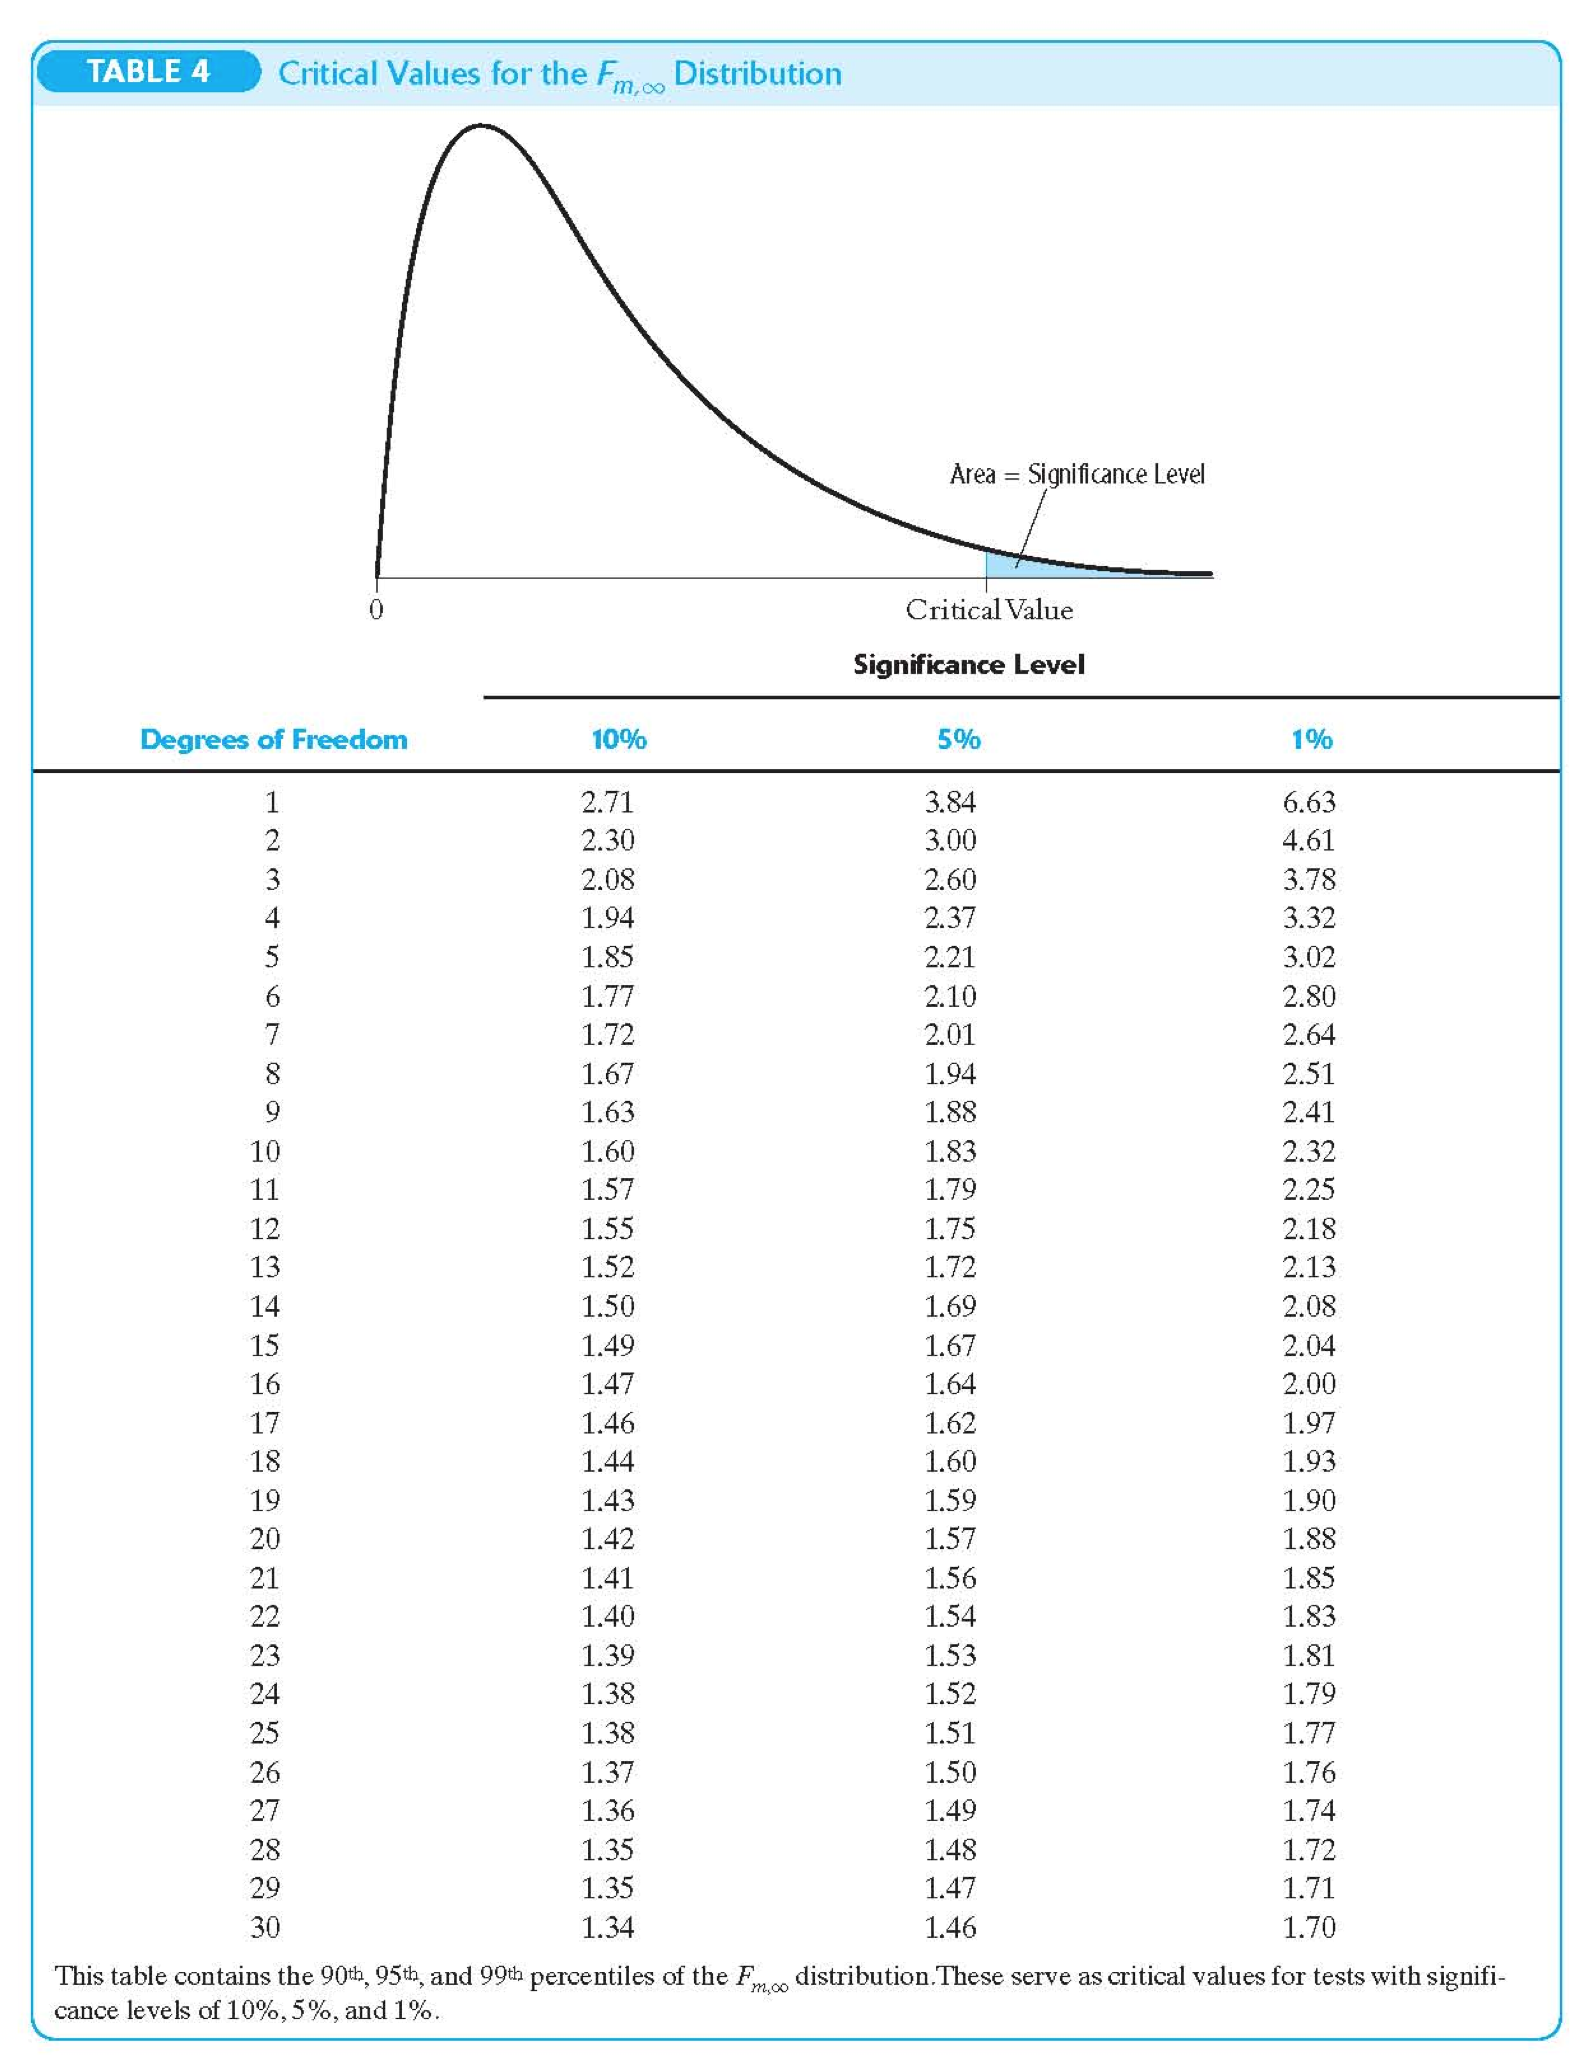
\includegraphics[width=0.8\textwidth]{img/fdist.png}
\caption{The table of critical values of the \(F(q, \infty)\) distribution}
\end{figure}
\end{column}

\begin{column}{0.5\columnwidth}
\begin{figure}[htbp]
\centering
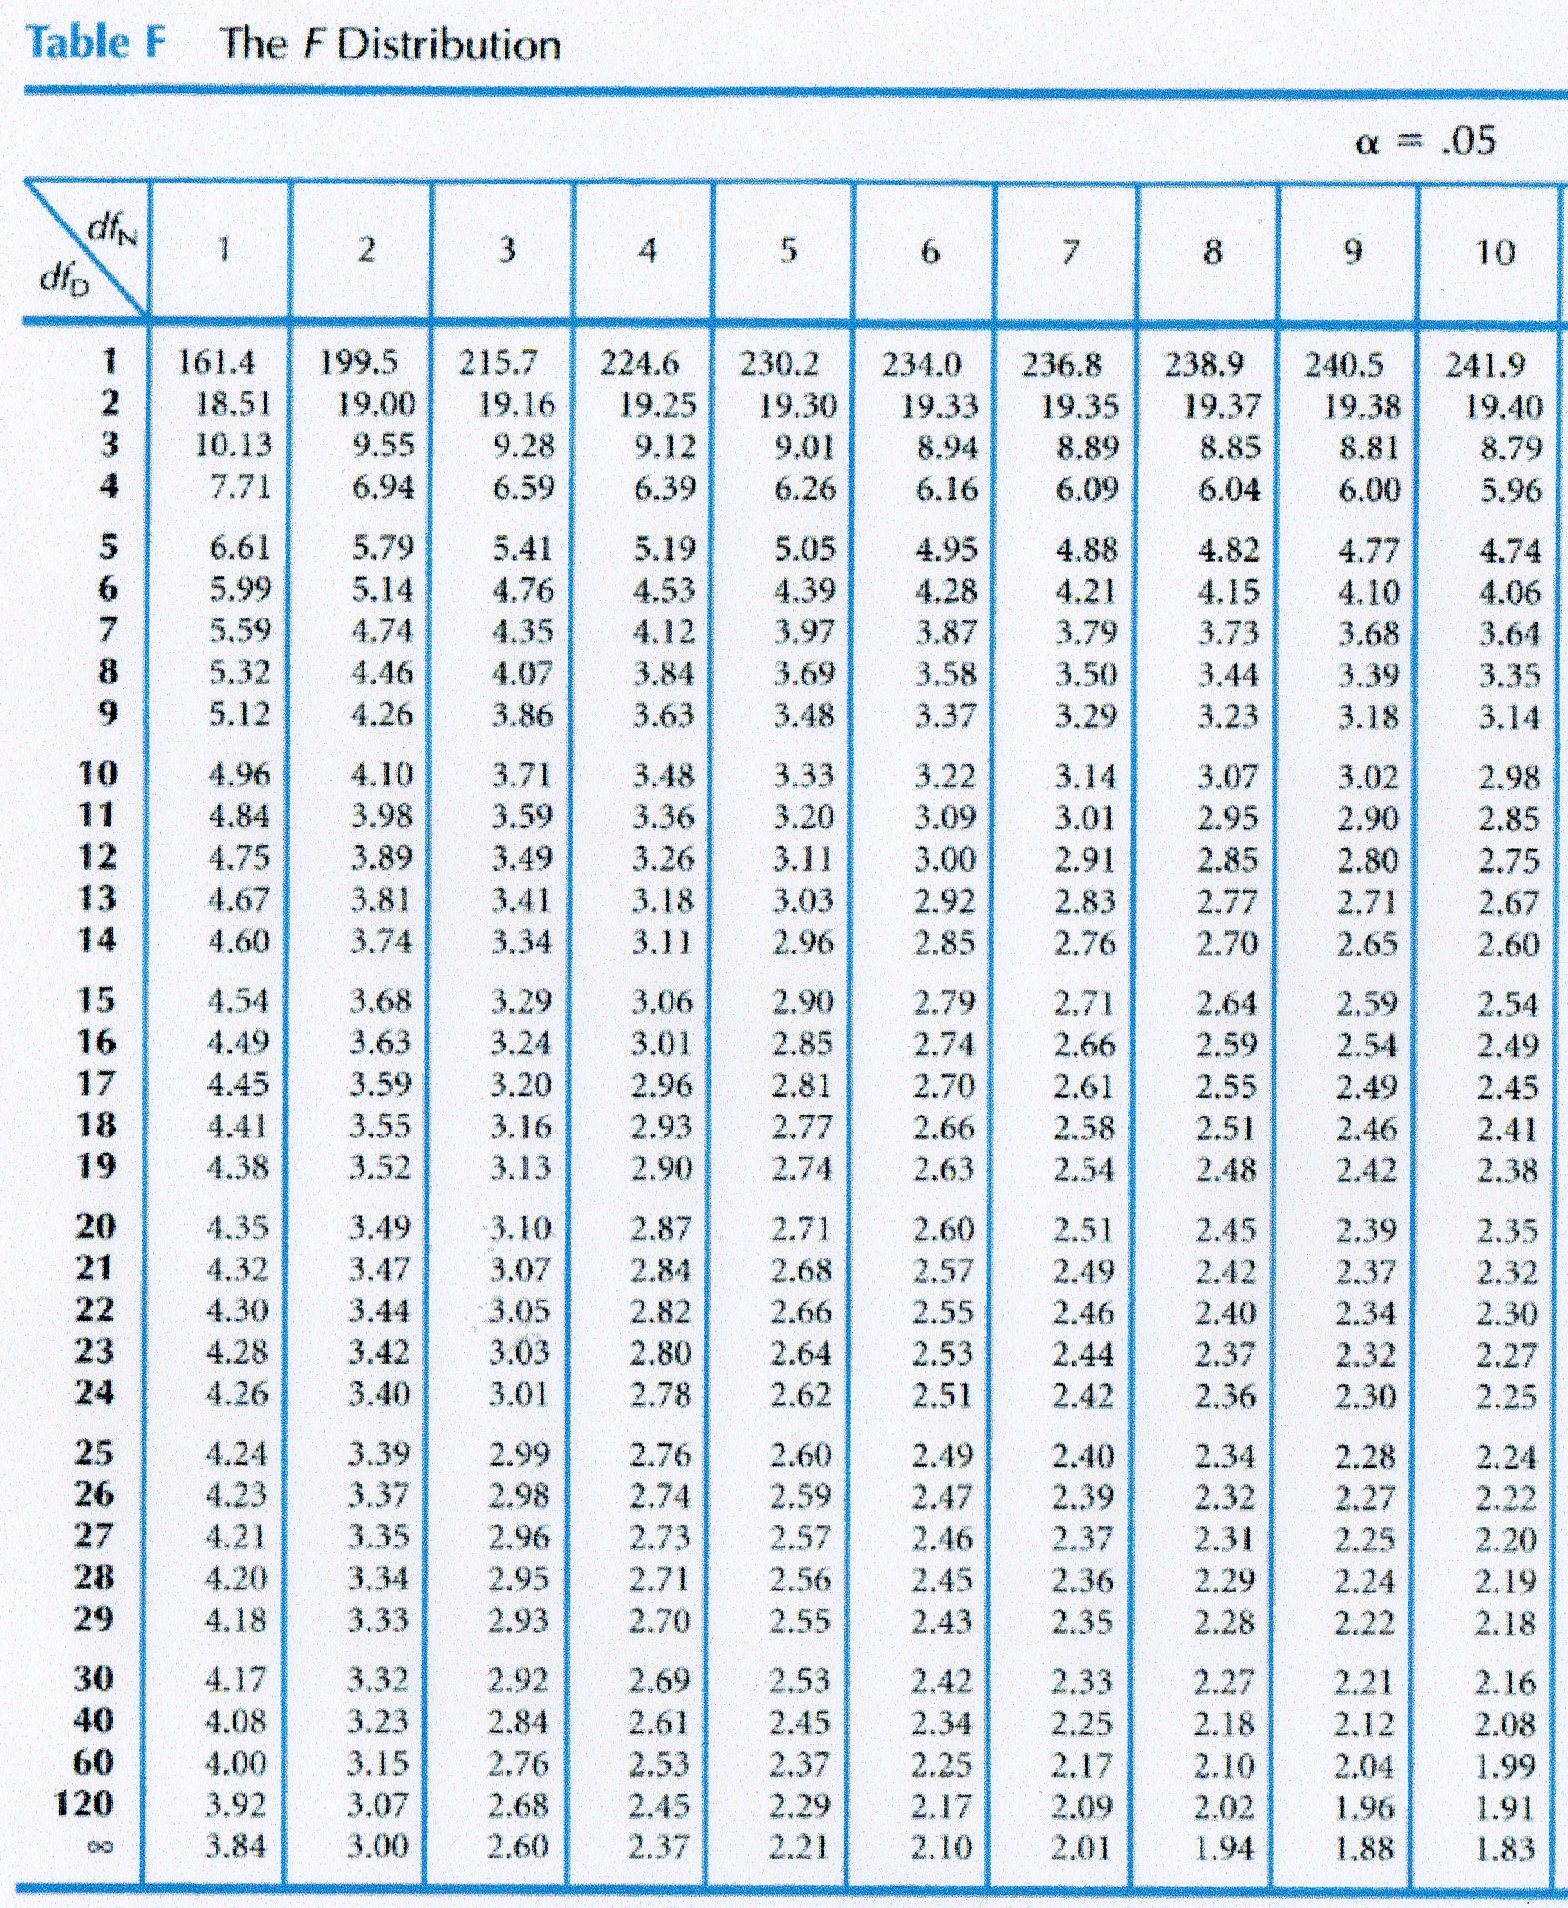
\includegraphics[width=0.8\textwidth]{img/Ftrunc.jpg}
\caption{The table of critical values at the 5\% level of the \(F(m, n)\) distribution}
\end{figure}
\end{column}
\end{columns}
\end{frame}

\section{Confidence Sets for multiple coefficients}
\label{sec:org1ee8fa0}
\setcounter{tocdepth}{1}
\tableofcontents[currentsection]
\begin{frame}[label={sec:org8579a42}]{Confidence set: definition}
A 95\% \alert{confidence set} for two or more coefficients is

\begin{itemize}
\item a set that contains the true population values of these coefficients
in 95\% of randomly drawn samples.

\item Equivalently, the set of coefficient values that cannot be rejected
at the 5\% significance level.
\end{itemize}
\end{frame}

\begin{frame}[label={sec:org54e3ab1}]{How to construct a confidence set}
Suppose that we construct the confidence set for \(\beta_1 =
\beta_{1,0}, \beta_2 = \beta_{2,0}\).

\begin{itemize}
\item Let \(F_{\beta_1, \beta_2}\) be the heteroskedasticity-robust or
homoskedasticity-only F-statistic.

\item A 95\% confidence set is
\[\{\beta_1, \beta_2:\, F_{\beta_1,\beta_2} < c_F\}\]
where \(c_F\) is the 5\% critical value of the \(F(2, \infty)\)
distribution, which is close to 3 in this case.

\item This set has coverage rate 95\% because the test on which it is based
has the size of 5\%.

\item Therefore the confidence set constructed as the nonrejected values
contains the true value 95\% of the time.
\end{itemize}
\end{frame}

\begin{frame}[label={sec:orgcd7a2a8}]{The confidence set based on the F-statistic is an ellipse}
\begin{itemize}
\item According to Equation (\ref{eq:ftest-q2}), the confidence set for \(\beta_1, \text{ and } \beta_2\) is
\begin{gather*}
\left\{ \beta_1, \beta_2:\, F = \frac{1}{2}\frac{t^2_1 + t^2_2 - 2 \hat{\rho}_{t_1,t_2}t_1t_2}{1 - \hat{\rho}_{t_1,t_2}^2} \leq 3 \right\}
\end{gather*}

\item Plugging the formula of \(t_1\) and \(t_2\), the F-statistic becomes
\begin{equation*}
\left[ \left(\frac{\hat{\beta}_1 - \beta_{1,0}}{SE(\hat{\beta}_1)}\right)^2 + \left(\frac{\hat{\beta}_2 - \beta_{2,0}}{SE(\hat{\beta}_2)}\right)^2 + 2 \hat{\rho}_{t_1,t_2}\left(\frac{\hat{\beta}_1 - \beta_{1,0}}{SE(\hat{\beta}_1)}\right) \left(\frac{\hat{\beta}_2 - \beta_{2,0}}{SE(\hat{\beta}_2)}\right) \right] \leq 3
\end{equation*}
\end{itemize}
\end{frame}

\begin{frame}[label={sec:org941fe2d}]{The confidence set: an illustration}
\begin{figure}[htbp]
\centering
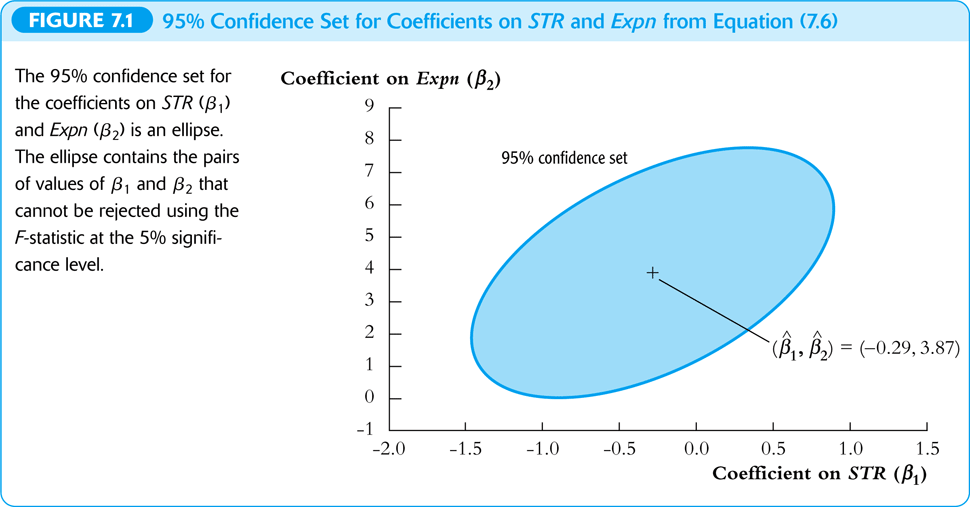
\includegraphics[width=.9\linewidth]{img/fig-7-1.png}
\caption{\label{fig:orgc2e52f5}
95\% Confidence Set for Coefficients on STR and Expn}
\end{figure}
\end{frame}

\section{Model Specification for Multiple Regression}
\label{sec:org253b2aa}
\setcounter{tocdepth}{1}
\tableofcontents[currentsection]
\begin{frame}[label={sec:org2b72b3d}]{Omitted variable bias in multiple regression}
\begin{itemize}
\item We should always be alert to omitted variable bias in the OLS
estimation.

\item For omitted variable bias to arise, two things must be true:
\begin{enumerate}
\item At least one of the included regressors must be correlated with the
omitted variable.
\item The omitted variable must be a determinant of the dependent
variable, \(Y\).
\end{enumerate}

\item With omitted variable bias, the least square assumption \(E(u|X) = 0\)
does not hold any more.
\end{itemize}
\end{frame}

\begin{frame}[label={sec:org923dcd8}]{The problem of the assumption of \(E(u|X) = 0\) and control variables}
\begin{itemize}
\item The assumption of \(E(u|X) = 0\) is essential to ensures unbiasedness
and consistency. However, it is too strong to be completely realized
in practice.

\item What we can do is that we divide all regressors into two groups:
\begin{enumerate}
\item One group consists of regressors whose causal effects on \(Y\) are our
research interest so that we want unbiased estimates of these
coefficients.
\item Another group consists of regressors whose causal effects on \(Y\) are
not our focus. But if we omit them, we would risk making omitted
variable bias in the coefficients that we do care.
\end{enumerate}

\item The regressors in the latter group are called \alert{control
variable}.

\item W use an assumption that is weaker than the assumption of
\(E(u|X)=0\) to ensure that the estimated coefficients on the
regressors in the first groups are unbiased, maintaining the causal
implication that we want.
\end{itemize}
\end{frame}

\begin{frame}[label={sec:orgdf993e5}]{Control variables: definition}
\begin{block}{Definition}
A control variable \(W\) is a variable that is correlated with, and
controls for, an omitted causal factor in the regression of Y on X,
but which itself does not necessarily have a causal effect on Y.
\end{block}

\begin{block}{The role of control variables}
A control variable is not the object of interest in the study; rather
it is a regressor included to hold constant factors that, if
neglected, could lead to the estimated causal effect of interest to
suffer from omitted variable bias.
\end{block}
\end{frame}

\begin{frame}[label={sec:orgbd390e1}]{The test score example}
\[TestScore = \underset{(5.6)}{700.2} - \underset{(0.27)}{1.00}STR -
\underset{(0.033)}{0.122}PctEL - \underset{(0.024)}{0.547}LchPct,\,
\bar{R}^2 = 0.773 \]

Where \(PctEL=\) percent English learners in the school district,
\(LchPct=\) percent of students receiving a free/subsidized lunch.

\begin{itemize}
\item Which variable is the variable of interest? \(STR\)
\item Which variables are control variables? Do they have causal
implications? What do they control for?
\end{itemize}
\end{frame}

\begin{frame}[label={sec:org86cdee4}]{What makes an effective control variable?}
\begin{itemize}
\item Three interchangeable statements about what makes an effective control
variable:
\begin{itemize}
\item An effective control variable is one which, when included in
the regression, makes the error term uncorrelated with the variable of
interest.
\item Holding constant the control variable(s), the variable of interest
is “as if” randomly assigned.
\item Among individuals (entities) with the same value of the control
variable(s), the variable of interest is uncorrelated with the
omitted determinants of \(Y\).
\end{itemize}

\item Control variables need not be causal, and their coefficients
generally do not have a causal interpretation.
\end{itemize}
\end{frame}

\begin{frame}[label={sec:org369f95f}]{Conditional mean independence: definition}
\begin{itemize}
\item \alert{Conditional mean independence}: given the
control variable, the mean of \(u_i\) doesn’t depend on the variable of
interest.
\end{itemize}

\vspace{0.2cm}

\begin{itemize}
\item Let \(X_i\) denote the variable of interest and \(W_i\) denote the control
variable(s).  \(W\) is an effective control variable if conditional mean
independence holds:
\[ E(u_i|X_i, W_i) = E(u_i|W_i) \]

\item Conditional mean independence substitute the first least square
assumption requiring \(E(u_i | X_i, W_i) = 0\).
\end{itemize}
\end{frame}

\begin{frame}[label={sec:orga53fed1}]{Implications of conditional mean independence}
Consider the regression model
\[ Y = \beta_0 + \beta_1 X + \beta_2 W + u \]
where \(X\) is the variable of interest and \(W\) is an effective control
variable so that conditional mean independence holds. In addition,
suppose that the other least square assumptions hold. Then,
\begin{itemize}
\item \(\beta_1\) has a causal interpretation.
\item \(\hat{\beta}_1\) is unbiased.
\item The coefficient on the control variable, \(\hat{\beta}_2\) is in
general biased.
\end{itemize}
\end{frame}

\begin{frame}[label={sec:org1486948}]{\(\beta_1\) has a causal interpretation}
The expected change in \(Y\) resulting from a change in \(X\), holding \(W\)
constant, is:
\begin{equation*}
\begin{split}
& E(Y|X = x + \Delta x, W = w) - E(Y|X = x, W = w) \\
&= \beta_0 + \beta_1(x + \Delta x) + \beta_2 w + E(u|X = x + \Delta x, W = w) \\
&\text{ } - \beta_0 + \beta_1 x + \beta_2 w + E(u|X = x, W = w) \\
&= \beta_1 \Delta x + \left( E(u|W = w) -  E(u|W = w) \right) \\
&= \beta_1 \Delta x
\end{split}
\end{equation*}
In the second equality, we use conditional mean independence \(E(u|X =
x + \Delta x, W = w) = E(u|X = x, W = w) = E(u|W = w)\).
\end{frame}

\begin{frame}[label={sec:org323e17e}]{\(\hat{\beta}_1\) is unbiased and \(\hat{\beta}_2\) is biased}
For convenience, suppose that \(E(u|W) = \gamma_0 + \gamma_1 W\). Thus,
under conditional mean independence, we have
\[ E(u|X,W) = E(u|W) = \gamma_0 + \gamma_1 W \]
Let \(v = u - E(u|W)\) so that
\[E(v|X, W) = E(u|X,W) - E(u|W) = 0 \]
Then, it follows that
\[ u = E(u|X,W) + v = \gamma_0 + \gamma_1 W + v \]
\end{frame}

\begin{frame}[label={sec:org27ce9e0}]{\(\hat{\beta}_1\) is unbiased and \(\hat{\beta}_2\) is biased (cont'd)}
Then, the original model \(Y = \beta_0 + \beta_1 X + \beta_2 W + u\)
becomes
\begin{equation}
\begin{split}
Y &= \beta_0 + \beta_1 X + \beta_2 W + \gamma_0 + \gamma_1 W + v \notag \\
&= (\beta_0 + \gamma_0) + \beta_1 X + (\beta_2 + \gamma_1) W + v \notag \\
&= \delta_0 + \beta_1 X + \delta_2 W + v
\end{split}
\end{equation}
where \(\delta_0 = \beta_0 + \gamma_0\) and \(\delta_2 = \beta_2 +
\gamma_2\).

What can we conclude from the new model?
\begin{itemize}
\item The new model satisfy \(E(v|X,W) = 0\) so that the OLS estimator of
\(\delta_0, \beta_1, \text{ and } \delta_2\) are unbiased.
\item The estimated coefficients in the original model are actually
\(\hat{\beta}_1\) and \(\hat{\delta}_2\), which we know that
\(E(\hat{\beta}_1) = \beta_1\) and \(E(\hat{\beta}_2) = \delta_2 \neq
  \beta_2\) in general.
\end{itemize}
\end{frame}

\begin{frame}[label={sec:org21da272}]{Model specification in theory and in practice}
The following steps are advocated to set up a regression model:

\begin{block}{Step 1: Set up a base specification}
A core or base set of regressors should be chosen using a
combination of expert judgment, economic theory, and knowledge of
how data were collected. The regression using this base set of
regressors is referred to as a \alert{base specification}. This step
involves the following consideration:
\begin{enumerate}
\item identifying the variable of interest.
\item thinking of the omitted causal effects that could result in omitted
variable bias.
\item including those omitted causal effects if you can. If you
can’t, include variables correlated with them that serve as
control variables.
\end{enumerate}
\end{block}
\end{frame}

\begin{frame}[label={sec:org0e09e73}]{Model specification in theory and in practice (cont'd)}
\begin{block}{Step 2: Set up alternative specifications}
Also specify a range of plausible \alert{alternative model
specifications}, which include additional candidate variables.
\begin{enumerate}
\item If the estimates of the coefficients of interest are numerically
similar across the alternative specifications, then this
provides evidence that the estimates from your base
specification are reliable.
\item If the estimates of the coefficients of interest change
substantially across specifications, this often provides
evidence that the original specification had omitted variable
bias.
\end{enumerate}
\end{block}
\end{frame}

\begin{frame}[label={sec:org8239c50}]{Model specification in theory and in practice (cont'd)}
\begin{block}{Step 3: Use test statistics to judge a model specification}
\begin{enumerate}
\item Use \(R^2\) and \(\bar{R}^2\) to see the overall goodness of fit of
a model specification. Caution: a high \(R^2\) or \(\bar{R}^2\) does
not mean that you have eliminated omitted variable bias. Neither
does a high \(R^2\) or \(\bar{R}^2\) mean that the included
variables and the model as a whole are statistically
significant.
\item Use t-statistic to check the significance of individual
coefficients, and use F-statistic to check the overall
significance of the model as a whole. That is, use F test for
\[H_0:\, \beta_1 = \beta_2 = \cdots = \beta_k = 0 \]
\end{enumerate}
\end{block}
\end{frame}

\begin{frame}[shrink,label={sec:org0da7a15}]{Analysis of the test score data set}
\begin{figure}[htbp]
\centering
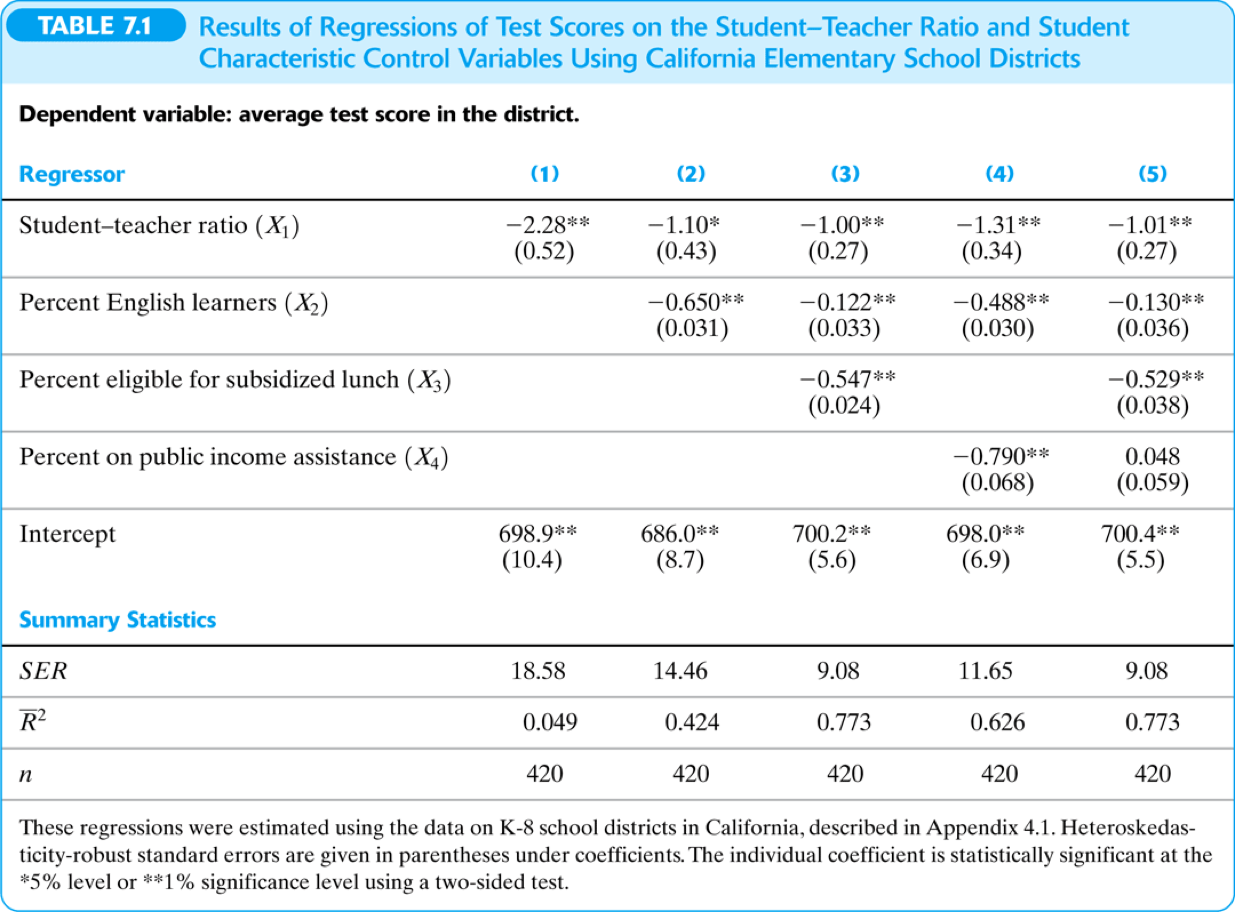
\includegraphics[width=.9\linewidth]{img/tab-7-1.png}
\end{figure}
\end{frame}
\end{document}